% Figure 4 -- cost landscape of the surveyed selectors (TikZ source; also provided as Figure_4_complexity.drawio)
% Exponents written next to the benchmarked methods are the measured alpha_n / alpha_p of E3 (e3_exponents_vs_table5.csv)
\documentclass[tikz,border=4pt]{standalone}
\usepackage{amsmath}\usepackage{helvet}\renewcommand{\familydefault}{\sfdefault}
\usetikzlibrary{positioning,arrows.meta,calc,shapes.geometric}
% Document information of the PDF (Author = Thu Nguyen); see Scripts/set_figure_metadata.py
\pdfinfo{/Author (Thu Nguyen) /Title (Fig. 4. Cost landscape of the surveyed gene selectors)}
\begin{document}
\footnotesize
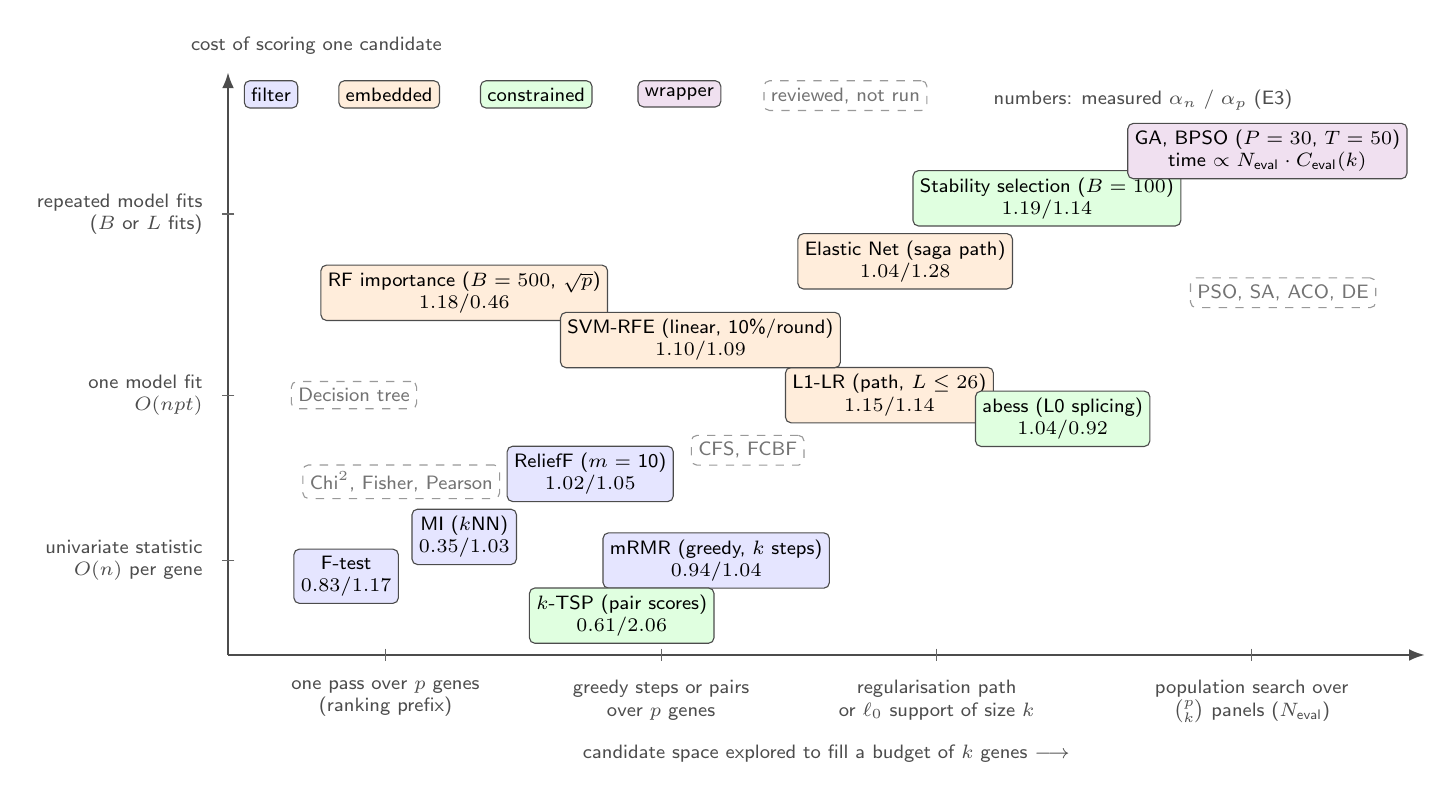
\begin{tikzpicture}[x=1cm,y=1cm,
  axis/.style={-{Latex[length=2mm]}, thick, black!70},
  m/.style={draw=black!70, fill=white, rounded corners=2pt, inner sep=2.5pt, font=\scriptsize, align=center},
  filter/.style={m, fill=blue!10},
  emb/.style={m, fill=orange!14},
  con/.style={m, fill=green!12},
  wrap/.style={m, fill=violet!12},
  notrun/.style={m, draw=black!40, text=black!55, dashed},
  lab/.style={font=\scriptsize, text=black!70, align=center}]

% axes
\draw[axis] (0,0) -- (15.2,0); \node[lab] at (7.6,-1.25) {candidate space explored to fill a budget of $k$ genes $\longrightarrow$};
\draw[axis] (0,0) -- (0,7.4) node[above right, lab, xshift=-6mm, yshift=1mm] {cost of scoring one candidate};
% x ticks
\foreach \x/\t in {2/{one pass over $p$ genes\\(ranking prefix)}, 5.5/{greedy steps or pairs\\over $p$ genes}, 9/{regularisation path\\or $\ell_0$ support of size $k$}, 13/{population search over\\$\binom{p}{k}$ panels ($N_{\text{eval}}$)}} {
  \draw[black!60] (\x,0.08) -- (\x,-0.08); \node[lab, below=1mm] at (\x,-0.1) {\t};
}
% y ticks
\foreach \y/\t in {1.2/{univariate statistic\\$O(n)$ per gene}, 3.3/{one model fit\\$O(npt)$}, 5.6/{repeated model fits\\($B$ or $L$ fits)}} {
  \draw[black!60] (0.08,\y) -- (-0.08,\y); \node[lab, left=1mm, align=right] at (-0.1,\y) {\t};
}
% filters
\node[filter] at (1.5,1.0) {F-test\\$0.83 / 1.17$};
\node[filter] at (3.0,1.5) {MI ($k$NN)\\$0.35 / 1.03$};
\node[filter] at (4.6,2.3) {ReliefF ($m$ = 10)\\$1.02 / 1.05$};
\node[filter] at (6.2,1.2) {mRMR (greedy, $k$ steps)\\$0.94 / 1.04$};
\node[notrun] at (2.2,2.2) {Chi$^2$, Fisher, Pearson};
\node[notrun] at (6.6,2.6) {CFS, FCBF};
% embedded
\node[emb] at (8.4,3.3) {L1-LR (path, $L \le 26$)\\$1.15 / 1.14$};
\node[emb] at (8.6,5.0) {Elastic Net (saga path)\\$1.04 / 1.28$};
\node[emb] at (3.0,4.6) {RF importance ($B = 500$, $\sqrt{p}$)\\$1.18 / 0.46$};
\node[emb] at (6.0,4.0) {SVM-RFE (linear, 10\%/round)\\$1.10 / 1.09$};
\node[notrun] at (1.6,3.3) {Decision tree};
% constrained
\node[con] at (10.6,3.0) {abess (L0 splicing)\\$1.04 / 0.92$};
\node[con] at (10.4,5.8) {Stability selection ($B = 100$)\\$1.19 / 1.14$};
\node[con] at (5.0,0.5) {$k$-TSP (pair scores)\\$0.61 / 2.06$};
% wrappers
\node[wrap] at (13.2,6.4) {GA, BPSO ($P = 30$, $T = 50$)\\time $\propto N_{\text{eval}} \cdot C_{\text{eval}}(k)$};
\node[notrun] at (13.4,4.6) {PSO, SA, ACO, DE};
% legend
\node[filter, anchor=north west] at (0.2,7.3) {filter};
\node[emb, anchor=north west] at (1.4,7.3) {embedded};
\node[con, anchor=north west] at (3.2,7.3) {constrained};
\node[wrap, anchor=north west] at (5.2,7.3) {wrapper};
\node[notrun, anchor=north west] at (6.8,7.3) {reviewed, not run};
\node[lab, anchor=north west, align=left] at (9.6,7.3) {numbers: measured $\alpha_n$ / $\alpha_p$ (E3)};
\end{tikzpicture}
\end{document}
